\documentclass[12pt, a4paper]{book}

\usepackage[english]{babel}
\usepackage[T1]{fontenc}
\usepackage[utf8]{inputenc}
\usepackage{lmodern}
\usepackage{listings}
\usepackage{tikz}
\usepackage{amsmath}
\usepackage{amssymb}
\usepackage{framed}
\usepackage{graphicx}
\usepackage{booktabs}

\graphicspath{{img/}}

\usetikzlibrary{arrows, chains, decorations}

\author{Florian Thuin}
\title{LSINF2224 - Programming methods}

\begin{document}
    \maketitle
    \tableofcontents
%%%%%%%%%%%%%%%%%%%%%%%%%%%%%%%%%%%%%%%%%%%%%%%%%%%%%%%%%%%%%%%%%%%%%%%%%%%%%%%%
% SECTION : Organization
%%%%%%%%%%%%%%%%%%%%%%%%%%%%%%%%%%%%%%%%%%%%%%%%%%%%%%%%%%%%%%%%%%%%%%%%%%%%%%%%
  \section{Organization}
  \label{sec:Organization}

  \subsection{Objectives}
  \label{sub:Objectives}
  \subsection{Synopsis}
  \label{sub:Synopsis}
  \subsection{Website}
  \label{sub:Website}
  \subsection{Course Outline}
  \label{sub:Course Outline}
  \subsection{Course material}
  \label{sub:Course material}
  \subsection{Bibliography}
  \label{sub:Bibliography}
  \subsection{Labs}
  \label{sub:Labs}
  \subsubsection{Goals}
  \label{subs:Goals}
  \subsubsection{Implementation}
  \label{subs:Implementation}
  \subsubsection{Languages}
  \label{subs:Languages}
  \subsubsection{Software}
  \label{subs:Software}
  \subsubsection{Assignments}
  \label{subs:Assignments}
  \subsection{Evaluation}
  \label{sub:Evaluation}


%%%%%%%%%%%%%%%%%%%%%%%%%%%%%%%%%%%%%%%%%%%%%%%%%%%%%%%%%%%%%%%%%%%%%%%%%%%%%%%%
% SECTION : Demonstration
%%%%%%%%%%%%%%%%%%%%%%%%%%%%%%%%%%%%%%%%%%%%%%%%%%%%%%%%%%%%%%%%%%%%%%%%%%%%%%%%
  \section{Demonstration}
  \label{sec:Demonstration}

  The goal of this initial demo is to show how we can automatically verify a
  Java program. We will use \textit{ESC/Java} that uses \textbf{enriched formal
  specifications} to make automated checks.

  \subsection{Binary Search: Implementation}
  \label{sub:Binary Search: Implementation}

  \lstinputlisting[language=Java, caption={Implementation of a binary search in
  Java}]{BinarySearch.java}

  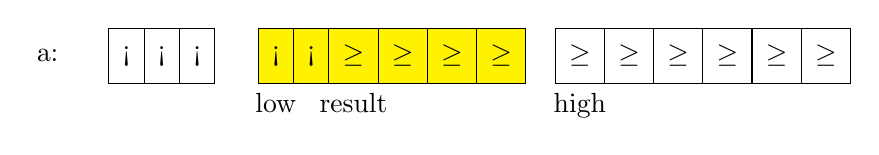
\begin{tikzpicture}
      \tikzstyle{element}=[rectangle, draw, inner sep=5pt, outer sep=0pt, minimum height=0.7cm]
      \draw (0,0) node(a) {a:};
      \node[element, right of=a] (b) {<};
      \node[element, right=0cm of b] (c) {<};
      \node[element, right=0cm of c] (d) {<};
      \node[element, right of=d, fill=yellow] (f) {<};
      \node[below=0cm of f] (low) {low};
      \node[element, right=0cm of f, fill=yellow] (g) {<};
      \node[element, right=0cm of g, fill=yellow] (h) {$\ge$};
      \node[below=0cm of h] (result) {result};
      \node[element, right=0cm of h, fill=yellow] (i) {$\ge$};
      \node[element, right=0cm of i, fill=yellow] (j) {$\ge$};
      \node[element, right=0cm of j, fill=yellow] (k) {$\ge$};
      \node[element, right of=k] (l) {$\ge$};
      \node[below=0cm of l] (high) {high};
      \node[element, right=0cm of l] (m) {$\ge$};
      \node[element, right=0cm of m] (n) {$\ge$};
      \node[element, right=0cm of n] (o) {$\ge$};
      \node[element, right=0cm of o] (p) {$\ge$};
      \node[element, right=0cm of p] (q) {$\ge$};
  \end{tikzpicture}

%%%%%%%%%%%%%%%%%%%%%%%%%%%%%%%%%%%%%%%%%%%%%%%%%%%%%%%%%%%%%%%%%%%%%%%%%%%%%%%%
%%%%%%%%%%%%%%%%%%%%%%%%%%%%%%%%%%%%%%%%%%%%%%%%%%%%%%%%%%%%%%%%%%%%%%%%%%%%%%%%
% CHAPTER : Foundations
%%%%%%%%%%%%%%%%%%%%%%%%%%%%%%%%%%%%%%%%%%%%%%%%%%%%%%%%%%%%%%%%%%%%%%%%%%%%%%%%
%%%%%%%%%%%%%%%%%%%%%%%%%%%%%%%%%%%%%%%%%%%%%%%%%%%%%%%%%%%%%%%%%%%%%%%%%%%%%%%%
  \chapter{Foundations}
  \label{chap:Foundations}

%%%%%%%%%%%%%%%%%%%%%%%%%%%%%%%%%%%%%%%%%%%%%%%%%%%%%%%%%%%%%%%%%%%%%%%%%%%%%%%%
% SECTION : Introduction
%%%%%%%%%%%%%%%%%%%%%%%%%%%%%%%%%%%%%%%%%%%%%%%%%%%%%%%%%%%%%%%%%%%%%%%%%%%%%%%%
  \section{Introduction}
  \label{sec:Introduction}

In this chapter, we will discuss the foundations of proofs, what can be done
and what cannot, why and how. \newline

The basis of this course are the programs. Every program has a language, the
language we will use is a mix between Java and Pascal (it should be very
easy for you to read it) that has a minimal set of interesting constructs
because we only need assignment, sequence, choice (conditions) and loops.
\newline

\paragraph{Example} computing $a^b$
\lstset{morekeywords={if,else,do,while}}
\begin{lstlisting}
stmt  ::= var=expr;
       |  {stmts}
       |  if (bexpr) then stmt else stmt
       |  while (bexpr) do stmt
stmts ::= stmt*
\end{lstlisting}

Each language has a syntax (the structure of program text), a static semantics
(typing, identifier scopes) that defines well-formed programs and a dynamic
semantics that defines the program behaviour (including runtime errors).
\newline

\begin{verbatim}
stmt  ::= var=expr;
       |  {stmts}
       |  if (bexpr) then stmt else stmt
       |  while (bexpr) do stmt
stmts ::= stmt*
\end{verbatim}

In this paper, we will only discuss well-formed programs without typing, and we
don't care about static semantics: no variable declaration, no types here.

  \begin{figure}[!ht]
      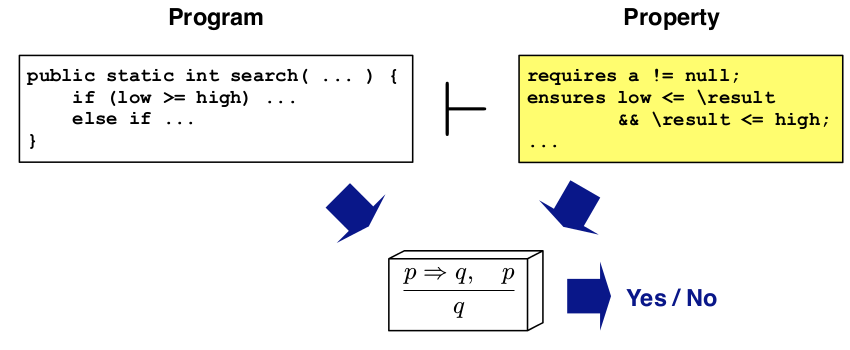
\includegraphics[width=\linewidth]{program_proofs.png}
      \caption{Program proofs}
  \end{figure}
%%%%%%%%%%%%%%%%%%%%%%%%%%%%%%%%%%%%%%%%%%%%%%%%%%%%%%%%%%%%%%%%%%%%%%%%%%%%%%%%
 % SECTION : Foundations
%%%%%%%%%%%%%%%%%%%%%%%%%%%%%%%%%%%%%%%%%%%%%%%%%%%%%%%%%%%%%%%%%%%%%%%%%%%%%%%%
  \section{Foundations}
  \label{sec:Foundations}

\subsection{Expressions}
\label{sub:Expressions}


Programs are made of \textit{expressions} that are each part that computes a
value. The syntax for expression is the following:

\begin{verbatim}
expr  ::= nexpr|bexpr|...
nexpr ::= number|var|-nexpr|nexpr+nexpr|...
bexpr ::= true|false|!bexpr|bexpr&&bexpr|...
\end{verbatim}

Expressions are weither \textit{numerical expression} $nexpr \subset expr$
($2,x, abs(y), a+b$) or boolean expressions $bexpr \subset expr$
($a[k]>0, x==2, empty(l)$). We will assume that each expression is well-typed
and pure (without side effect\footnote{Side effects are modifications of global
variables or static variables or interaction with the world that may lead to
variation between executions}). \newline

\subsection{Execution state}
\label{sub:Execution state}

\begin{figure}[!ht]
    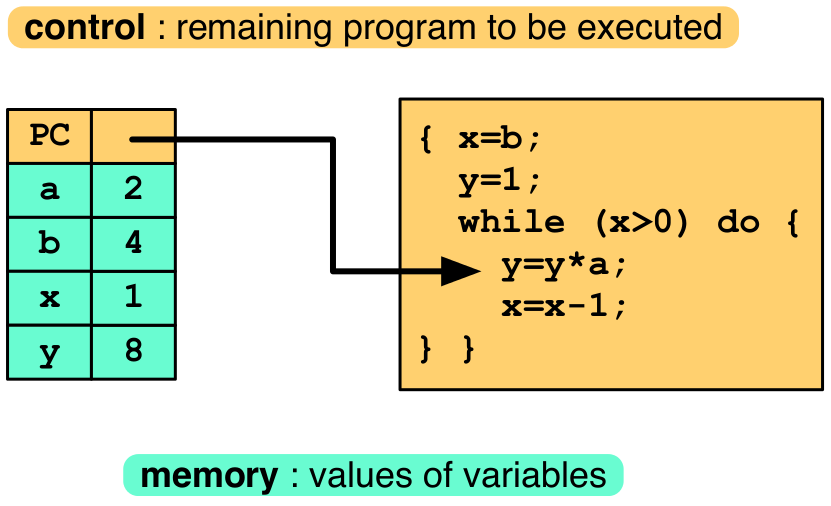
\includegraphics[width=\linewidth]{execution_state.png}
    \caption{Execution state}
\end{figure}

\paragraph{How do we store states?} We know the value of the variables (the
result of evaluating expressions as integer or boolean in our examples). The
set of data values $D$ for each state contains all the boolean
$b \in B = {true, false}$, such that $B \subset D$. \newline

Those data values $d \in D$ are stored in \textit{stores} (memory) that are
functions that maps variables to their values. $\sigma$ is a store, $\Sigma$ is
the set of all the functions from the variables to their domains, $var$ is a
variable such that $\sigma \in \Sigma = var \rightarrow D$ with $\sigma(V)$ the
value of $V$ in $\sigma$.

\begin{minipage}{\linewidth}
    \begin{minipage}{0.4\linewidth}
        $$\sigma(a) = 2$$
        $$\sigma(y)=8$$
    \end{minipage}
    \begin{minipage}{0.4\linewidth}
        \centering
        \begin{tabular}{ll}
            \toprule
            a & 2 \\
            \midrule
            b & 4 \\
            \midrule
            x & 1 \\
            \midrule
            y & 8 \\
            \bottomrule
        \end{tabular}
    \end{minipage}
\end{minipage}

We can update the stores by modifying the value of the variables that we
write $\sigma[V := d] = \sigma'$ such that

\begin{itemize}
    \item $\sigma'(V') = d$ when $V' =V$
    \item $\sigma'(V') = \sigma(V')$ otherwise.
\end{itemize}

\begin{minipage}{\linewidth}
    \begin{minipage}{0.4\linewidth}
        $$\sigma[y := 16]$$
    \end{minipage}
    \begin{minipage}{0.4\linewidth}
        \centering
        \begin{tabular}{ll}
            \toprule
            a & 2 \\
            \midrule
            b & 4 \\
            \midrule
            x & 1 \\
            \midrule
            y & \textcolor{red}{16} \\
            \bottomrule
        \end{tabular}
    \end{minipage}
\end{minipage}

A \textbf{control state} is the program (or the residual program) to be executed
denoted $S \in stmt$. A \textbf{global state} is a \textit{configuration}, i.e.
an abstract machine about to execute a program $S$ from a store $\sigma$,
denoted $(S,\sigma) \in stmt \times \Sigma$ (or control $\times$ store).

\begin{figure}[!ht]
    \centering
    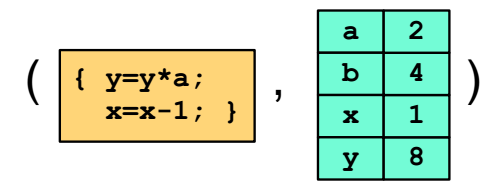
\includegraphics[width=\linewidth]{global_state.png}
    \caption{Representation of a global state}
\end{figure}

\subsection{Semantics}
\label{sub:Semantics}

In this part, we will describe the semantics used for expressions and boolean
expressions. \newline

As we consider expression in programs (only \textit{pure}\footnote{that does
not have a side-effect} expression where $\sigma$ does not change), we have to
extend $\sigma : V \rightarrow D$ to a valuation on $expr$:

$$
\sigma : expr \rightarrow D
$$

\begin{eqnarray}
    \textcolor{red}{\sigma(}\textcolor{green!60!black}{42}\textcolor{red}{)} & = & \textcolor{red}{42} \\
    \textcolor{red}{\sigma(}\textcolor{green!60!black}{true}\textcolor{red}{)} & = & \textcolor{red}{true} \\
    \textcolor{red}{\sigma(}\textcolor{green!60!black}{E1*E2}\textcolor{red}{)} & = & \textcolor{red}{\sigma(}\textcolor{green!60!black}{E1}\textcolor{red}{) \times \sigma(}\textcolor{green!60!black}{E2}\textcolor{red}{)} \\
    \textcolor{red}{\sigma(}\textcolor{green!60!black}{E1<=E2}\textcolor{red}{)} & = & \textcolor{red}{\sigma(}\textcolor{green!60!black}{E1}\textcolor{red}{) \le \sigma(}\textcolor{green!60!black}{E2}\textcolor{red}{)}
\end{eqnarray}

The parts in \textcolor{green!60!black}{green} are syntax, the parts in
\textcolor{red}{red} are semantics. \newline

For a boolean expression $B \in bexpr$, we define semantics as follow:

\begin{itemize}
    \item $[[B]] = \{\sigma \mid \sigma(B)\}$ is the set of stores in which $B$
    is true.
    \item $[[\lnot B]] = \{\sigma \mid \lnot \sigma(B)\}$ is the set of stores
    in which $B$ is false.
\end{itemize}

For example,
$$
\textcolor{red}{[[}\textcolor{green!60!black}{E1<=E2}\textcolor{red}{]] = \{\sigma \mid \sigma(}\textcolor{green!60!black}{E1}\textcolor{red}{) \le \sigma(}\textcolor{green!60!black}{E2}\textcolor{red}{)\}}
$$

\subsection{Transition}
\label{sub:Transition}

We define a \textbf{transition relation} $\longrightarrow$ between
configurations :

$$(S,\sigma) \longrightarrow (S',\sigma')$$

means:

\begin{itemize}
    \item executions of one step of $S$ from $\sigma$ yields $\sigma'$
    \item $S'$ being the remainder of $S$ after that step
\end{itemize}

The transition relation $\longrightarrow$ defines an \textbf{operational
semantics} for programs. The operational semantics will help us to know the
meaning of the instructions step-by-step and thus to get from \textit{pre} to
\textit{post}.

\begin{figure}[!ht]
    \centering
    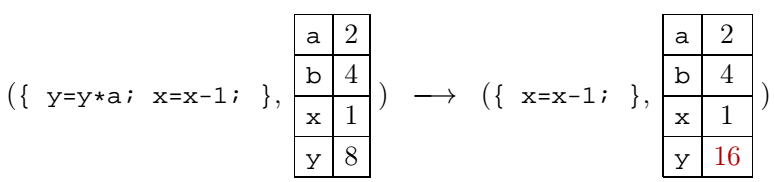
\includegraphics[width=\linewidth]{transition1.png}
    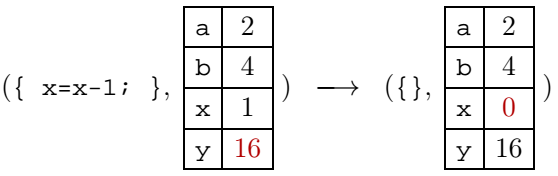
\includegraphics[width=\linewidth]{transition2.png}
    \caption{Transitions: Example}
\end{figure}

The transition relation is defined by \textit{induction} on program structure as
\textbf{inference rules}. \newline

\paragraph{Example} The instruction block $\{S_1 S_2 \ldots S_n\}$

\begin{itemize}
    \item IF $(S_1, \sigma) \longrightarrow (S_{1}^{'},\sigma')$ THEN
    $(\{S_1S_2\ldots S_n\}, \sigma) \longrightarrow (\{S_1^{'}S_2\ldots S_n\},\sigma')$
    \item IF $S_1 = \{\}$ (i.e. $S_1$ is done) THEN $(\{S_1S_2\ldots S_n\},\sigma) \longrightarrow (\{S_2\ldots S_n\}, \sigma)$
\end{itemize}

This is a \textbf{structural operational semantics} (SOS).

\subsection{Inference}
\label{sub:Inference}

Now that we have the semantics with us, we will need rules to decide the value
of the next state. We denote an inference rule as:

$$\frac{\phi_{1} \ldots \phi_{n}}{\phi}$$

which means that

\begin{itemize}
    \item if $\phi_1$ and \ldots and $\phi_n$ then $\phi$
    \item from $\phi_1$ and \ldots and $\phi_n$ we can deduce $\phi$
\end{itemize}

Example:

$$
\frac{(S,\sigma) \longrightarrow (S', \sigma')}
{(\{S\ SS\},\sigma) \longrightarrow (\{S'\ SS\}, \sigma')}
$$

Axioms are particular cases of rules, because they are \textit{true} without
condition. We denote them as:

$$
\frac{}
{\ \phi \ }
$$

which means

\begin{itemize}
    \item $\phi$ is true
    \item $\phi$ is an axiom
\end{itemize}

Example:
$$
\frac{}
{(\{ \{ \} \ SS, \sigma \}) \longrightarrow (\{ SS \}, \sigma)}
$$
means that the \textit{empty program} followed by a sequence of instructions can
be reduced to this sequence of instructions. \newline

An \textbf{inference system} is a set of inference rules $R$ including axioms.
Axioms and inference rules can be derivated to discover new rules that will lead
to the searched proof. \newline

A \textbf{derivation} of $\phi$ in $R$ (denoted $\vdash_R \phi$) is a sequence
of formulae $\phi_0,\phi_1,\ldots,\phi_n$ ending with $\phi_n \equiv \phi$ such
that each formula $\phi_k$ results from applying a rule of $R$ to preceding
formulae $\phi_l$ with $l<k$. \newline

We can formalize the construction by derivation from $R^0$ (the set of axioms):

\begin{eqnarray}
R^{0}   & = & \{\phi \mid \frac{}{\ \phi \ } \exists R\} \\
R^{k+1} & = & R^{k} \cup \{ \phi \mid \frac{\phi_{1} \ldots \phi_{n}}{\phi}
\in R \land \phi_{1}\ldots\phi_{n} \in R^{k} \} \\
R^{*}   & = & \bigcup_{k} R^{k}
\end{eqnarray}

$$
\vdash_{R} \phi \iff \phi \in R^{*}
$$

\subsection{Transition rules as inference rules}
\label{sub:Transition rules as inference rules}

In this part, we will write down transition rules as inference rules. We will
do it for each element of our language: assignment, sequence, condition
(choice), loop.

\paragraph{Assignment V=E;}

$$
\frac{}
{(V=E;,\sigma) \longrightarrow (\{ \}, \sigma [V := \sigma (E)] )}
$$

\paragraph{Sequence \{S SS\}} (S in the instruction, SS is the residual program
to be executed)

$$
\frac{(S,\sigma) \longrightarrow (S',\sigma')}
{(\{ S\ SS \} , \sigma ) \longrightarrow (\{S'\ SS\}, \sigma')}
$$

$$
\frac{}
{(\{ \{ \} SS\}, \sigma) \longrightarrow (\{ SS \}, \sigma)}
$$

\noindent \textbf{Condition} \verb#if# $(B)$ \verb#then# $S_{1}$ \verb#else# $S_{2}$

$$
\frac{}
{(\textrm{if } (B) \textrm{ then } S_{1} \textrm{ else } S_{2}, \sigma) \longrightarrow (S_{1}, \sigma)}
\ \sigma(B)
$$

$$
\frac{}
{(\textrm{if } (B) \textrm{ then } S_{1} \textrm{ else } S_{2}, \sigma) \longrightarrow (S_{2}, \sigma)}
\ \lnot\sigma(B)
$$

\noindent \textbf{Loop} \verb#while# (B) \verb#do# S

$$
\frac{}
{(\textrm{while } (B) \textrm{ do } S, \sigma) \longrightarrow (\{ S \textrm{ while } (B) \textrm{ do } S\}, \sigma)}
\sigma(B)
$$

$$
\frac{}
{(\textrm{while } (B) \textrm{ do } S, \sigma) \longrightarrow (\{ \}, \sigma)}
\lnot\sigma(B)
$$

\subsection{Runs, Termination, Divergence}

A program terminates iff the execution leads to the empty program (an empty
sequence of instructions). \newline

$(S_{0}, \sigma_{0}) \longrightarrow^{*} (S_{k}, \sigma_{k})$ iff there is a
\underline{finite} sequence

$$
(S_{0}, \sigma_{0}) \longrightarrow (S_{1}, \sigma_{1}) \longrightarrow \ldots
\longrightarrow (S_{k}, \sigma_{k})
$$

$(S, \sigma)$ terminates in $\sigma'$ iff $(S, \sigma) \longrightarrow^{*} (\{\}, \sigma')$ (with $\longrightarrow^{*}$ meaning a finite number of steps)

$(S_{0}, \sigma_{0}) \longrightarrow^{\omega}$ iff there is an \underline{infinite} sequence ($\omega$ means infinite enumerable)

$$
(S_{0}, \sigma_{0}) \longrightarrow (S_{1}, \sigma_{1}) \longrightarrow \ldots
$$

$(S,\sigma)$ diverges iff $(S,\sigma) \longrightarrow^{\omega}$

\paragraph{Semantics: Partial Correctness}

We define the semantics of a program $S$ as a function $[[S]]: \sum \rightarrow 2^{\Sigma}$ \newline

initial store $\rightarrow$ final store \newline

Partial correctness semantics:
$$
[[S]](\sigma) = \{\sigma' \mid (S,\sigma) \longrightarrow^{*} (\{\}, \sigma')\}
$$
where $[[S]](\sigma)$ is the set of possible final stores after executing $S$
from $\sigma$

\paragraph{Semantics (Set-Based Version)}

For convenience, it is useful to define $[[S]]$ on sets of initial states. \newline

For a set of stores $X \subseteq \Sigma$,
$$
[[S]](X) = \bigcup_{\sigma \in X} [[S]](\sigma)
$$

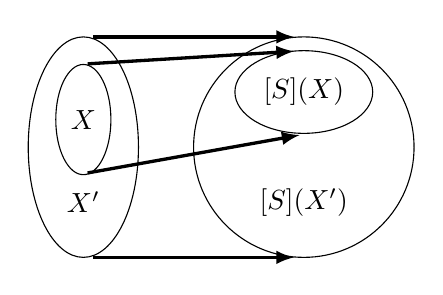
\begin{tikzpicture}[scale=0.7]
  \tikzstyle{suite}=[->,>=stealth’,thick,rounded corners=4pt]

  \draw (1,1) ellipse (1 and 2); % Right big ellipse
  \draw (1,1.5) ellipse (0.5 and 1); % Right little ellipse
  \node (A) at (1, 1.5) {$X$};
  \node (B) at (1, 0.0) {$X'$};
  \draw (5, 1) circle (2); % Right circle
  \draw (5, 2) ellipse (1.25 and 0.75); % Right ellipse in circle
  \node (C) at (5, 2) {$[S](X)$};
  \node (D) at (5, 0) {$[S](X')$};
  \node (E) at (1, 3) {}; % Top-left node
  \node (F) at (5, 3) {}; % Top-right node
  \draw[->,>=latex, very thick] (E)--(F); % Top arrow
  \node (G) at (1,-1) {};
  \node (H) at (5,-1) {};
  \draw[->,>=latex, very thick] (G)--(H); % Bottom arrow
  \node (I) at (0.9, 2.5) {};
  \node (J) at (5, 2.75) {};
  \draw[->,>=latex, very thick] (I)--(J); % Top-ellipse arrow
  \node (K) at (0.9, 0.5) {};
  \node (L) at (5.1, 1.25) {};
  \draw[->,>=latex, very thick] (K)--(L); % Bottom-ellipse arrow
\end{tikzpicture}

\paragraph{Property}: [[S]] is monotonic:

$$
X \subseteq X' \Rightarrow [[S]](X) \subseteq [[S]](X')
$$

\noindent Proof: obvious from definition \newline

Important for convergence of iterative computations \newline

\paragraph{Semantics: Total Correctness}

Distinguished value $\perp$ (bottom) denotes absence of final state (i.e.
the final state of a non-terminating program).

\textbf{Total Correctness Semantics:}
$$
{[[S]]}_{\perp}(\sigma) = [[S]](\sigma) \cup \{\perp \mid (S,\sigma) \longrightarrow^{\omega}\}
$$

${[[S]]}_{\perp}(\sigma)$ is like $[[S]](\sigma)$ plus $\perp$ if $S$ may
diverge from $\sigma$

\paragraph{Semantics: Determinism}

with the language defined so far, programs are deterministic and non-blocking.
If $S \neq \{ \}$, then there is one unique $(S',\sigma')$ such that
$(S,\sigma) \longrightarrow (S', \sigma')$. \newline

Hence $\lvert [[S]](\sigma) \rvert \le 1$ and $\lvert {[[S]]}_{\perp}(\sigma) \rvert = 1$. \\
If $S$ terminates, then $[[S]](\sigma) = {[[S]]}_{\perp}(\sigma) = \{\sigma'\}, \sigma' \neq \perp$ \\
If $S$ diverges, then $[[S]](\sigma) = \emptyset$ and ${[[S]]}_{\perp}(\sigma) = \{\perp\}$. \\
This is not true later with non-deterministic choice and concurrency.

\paragraph{Denotational Semantics}

$[[S]] : \Sigma \rightarrow 2^{\Sigma}$ is a denotation of the semantics of
program S, a mathematical object that fully describes the meaning of $S$.

\textbf{Denotational semantics} defines $[[[S]]](\sigma)$ by induction on $S$,
without resorting to the transition relation.

\begin{framed}
    \textbf{Example} : if-then-else
    $$
    [[\textrm{if } (B) \textrm{ then } S_{1} \textrm{ else } S_{2}]](X) =
    ([[S_{1}]] (X \cap [[B]])) \cup ([[S_{2}]] ( X \cap [[\lnot B]] ))
    $$
\end{framed}

In this course, we will consider operational semantics only.


%%%%%%%%%%%%%%%%%%%%%%%%%%%%%%%%%%%%%%%%%%%%%%%%%%%%%%%%%%%%%%%%%%%%%%%%%%%%%%%%
%%%%%%%%%%%%%%%%%%%%%%%%%%%%%%%%%%%%%%%%%%%%%%%%%%%%%%%%%%%%%%%%%%%%%%%%%%%%%%%%
% CHAPTER : Program proofs
%%%%%%%%%%%%%%%%%%%%%%%%%%%%%%%%%%%%%%%%%%%%%%%%%%%%%%%%%%%%%%%%%%%%%%%%%%%%%%%%
%%%%%%%%%%%%%%%%%%%%%%%%%%%%%%%%%%%%%%%%%%%%%%%%%%%%%%%%%%%%%%%%%%%%%%%%%%%%%%%%

  \chapter{Program Proofs}
  \label{chap:Program Proofs}

%%%%%%%%%%%%%%%%%%%%%%%%%%%%%%%%%%%%%%%%%%%%%%%%%%%%%%%%%%%%%%%%%%%%%%%%%%%%%%%%
% SECTION : Sequential programs
%%%%%%%%%%%%%%%%%%%%%%%%%%%%%%%%%%%%%%%%%%%%%%%%%%%%%%%%%%%%%%%%%%%%%%%%%%%%%%%%
  \section{Sequential Programs}
  \label{sec:Sequential Programs}

%%%%%%%%%%%%%%%%%%%%%%%%%%%%%%%%%%%%%%%%%%%%%%%%%%%%%%%%%%%%%%%%%%%%%%%%%%%%%%%%
% SECTION : Verification conditions
%%%%%%%%%%%%%%%%%%%%%%%%%%%%%%%%%%%%%%%%%%%%%%%%%%%%%%%%%%%%%%%%%%%%%%%%%%%%%%%%
  \section{Verification Conditions}
  \label{sec:Verification Conditions}
%%%%%%%%%%%%%%%%%%%%%%%%%%%%%%%%%%%%%%%%%%%%%%%%%%%%%%%%%%%%%%%%%%%%%%%%%%%%%%%%
% SECTION : Procedures
%%%%%%%%%%%%%%%%%%%%%%%%%%%%%%%%%%%%%%%%%%%%%%%%%%%%%%%%%%%%%%%%%%%%%%%%%%%%%%%%
  \section{Procedures}
  \label{sec:Procedures}

%%%%%%%%%%%%%%%%%%%%%%%%%%%%%%%%%%%%%%%%%%%%%%%%%%%%%%%%%%%%%%%%%%%%%%%%%%%%%%%%
% SECTION : Recursion
%%%%%%%%%%%%%%%%%%%%%%%%%%%%%%%%%%%%%%%%%%%%%%%%%%%%%%%%%%%%%%%%%%%%%%%%%%%%%%%%
  \section{Recursion}
  \label{sec:Recursion}

%%%%%%%%%%%%%%%%%%%%%%%%%%%%%%%%%%%%%%%%%%%%%%%%%%%%%%%%%%%%%%%%%%%%%%%%%%%%%%%%
% SECTION : Data Structures
%%%%%%%%%%%%%%%%%%%%%%%%%%%%%%%%%%%%%%%%%%%%%%%%%%%%%%%%%%%%%%%%%%%%%%%%%%%%%%%%
  \section{Data Structures}
  \label{sec:Data Structures}

  \section{Data abstraction}
  \label{sec:Data abstraction}


%%%%%%%%%%%%%%%%%%%%%%%%%%%%%%%%%%%%%%%%%%%%%%%%%%%%%%%%%%%%%%%%%%%%%%%%%%%%%%%%
% SECTION : Reactive Programs
%%%%%%%%%%%%%%%%%%%%%%%%%%%%%%%%%%%%%%%%%%%%%%%%%%%%%%%%%%%%%%%%%%%%%%%%%%%%%%%%
  \section{Reactive Programs}
  \label{sec:Reactive Programs}
  \subsection{From application to reactive}
  \label{sub:From application to reactive}
  \subsubsection{Applicative programs}
  \label{subs:Applicative programs}
  \subsubsection{Reactive programs}
  \label{subs:Reactive programs}
  \subsubsection{Prooofs of reactive programs}
  \label{subs:Prooofs of reactive programs}
  \subsection{Non-deterministic programs}
  \label{sub:Non-deterministic programs}
  \subsubsection{Guarded commands}
  \label{subs:Guarded commands}
  \subsubsection{Deadlock}
  \label{subs:Deadlock}
  \subsubsection{Strong vs. weak total correctness}
  \label{subs:Strong vs. weak total correctness}
  \subsection{Concurrent programs}
  \label{sub:Concurrent programs}
  \subsubsection{Interleaving}
  \label{subs:Interleaving}
  \subsubsection{Atomicity}
  \label{subs:Atomicity}
  \subsubsection{Disjoint parallel programs}
  \label{subs:Disjoint parallel programs}
  \subsubsection{Compositional proofs}
  \label{subs:Compositional proofs}
  \subsubsection{General concurrent programs}
  \label{subs:General concurrent programs}
  \subsubsection{Interference-free proofs}
  \label{subs:Interference-free proofs}
  \subsubsection{Fairness}
  \label{subs:Fairness}


%%%%%%%%%%%%%%%%%%%%%%%%%%%%%%%%%%%%%%%%%%%%%%%%%%%%%%%%%%%%%%%%%%%%%%%%%%%%%%%%
%%%%%%%%%%%%%%%%%%%%%%%%%%%%%%%%%%%%%%%%%%%%%%%%%%%%%%%%%%%%%%%%%%%%%%%%%%%%%%%%
% CHAPTER : Program validation
%%%%%%%%%%%%%%%%%%%%%%%%%%%%%%%%%%%%%%%%%%%%%%%%%%%%%%%%%%%%%%%%%%%%%%%%%%%%%%%%
%%%%%%%%%%%%%%%%%%%%%%%%%%%%%%%%%%%%%%%%%%%%%%%%%%%%%%%%%%%%%%%%%%%%%%%%%%%%%%%%

  \chapter{Program Validation}
  \label{chap:Program Validation}

%%%%%%%%%%%%%%%%%%%%%%%%%%%%%%%%%%%%%%%%%%%%%%%%%%%%%%%%%%%%%%%%%%%%%%%%%%%%%%%%
% SECTION : State-Based Models
%%%%%%%%%%%%%%%%%%%%%%%%%%%%%%%%%%%%%%%%%%%%%%%%%%%%%%%%%%%%%%%%%%%%%%%%%%%%%%%%
  \section{State-Based Models}
  \label{sec:State-Based Models}
  \subsection{Introduction}
  \label{sub:Introduction}
  \subsection{Summary}
  \label{sub:Summary}
  \subsection{Models of Reactive Programs?}
  \label{sub:Models of Reactive Programs?}
  \subsection{State machines}
  \label{sub:State machines}
  \subsubsection{Principles}
  \label{subs:Principles}
  \subsubsection{Definition}
  \label{subs:Definition}
  \subsubsection{Example}
  \label{subs:Example}
  \subsubsection{Traces}
  \label{subs:Traces}
  \subsection{Infinite executions}
  \label{sub:Infinite executions}
  \subsubsection{Example of State Machine}
  \label{subs:Example of State Machine}
  \subsection{State machines and programs}
  \label{sub:State machines and programs}
  \subsubsection{Example of Program}
  \label{subs:Example of Program}
  \subsubsection{Interpreted State Machines}
  \label{subs:Interpreted State Machines}
  \subsection{Kripke structure}
  \label{sub:Kripke structure}
  \subsubsection{Example}
  \label{subs:Example}
  \subsubsection{Interpretation on Programs}
  \label{subs:Interpretation on Programs}
  \subsection{Program Locations}
  \label{sub:Program Locations}
  \subsection{Temporal logic}
  \label{sub:Temporal logic}
  \subsection{LTL}
  \label{sub:LTL}
  \subsubsection{Principle}
  \label{subs:Principle}
  \subsubsection{Syntax}
  \label{subs:Syntax}
  \subsubsection{Semantics over traces}
  \label{subs:Semantics over traces}
  \subsubsection{Semantics over structures}
  \label{subs:Semantics over structures}
  \subsubsection{Examples (safety)}
  \label{subs:Examples (safety)}
  \subsubsection{Examples (liveness)}
  \label{subs:Examples (liveness)}
  \subsubsection{Examples (deadlock)}
  \label{subs:Examples (deadlock)}
  \subsubsection{Until vs Unless}
  \label{subs:Until vs Unless}
  \subsubsection{Quid of Hoare Logic?}
  \label{subs:Quid of Hoare Logic?}
  \subsubsection{Examples (pre/post)}
  \label{subs:Examples (pre/post)}
  \subsection{Other temporal logics}
  \label{sub:Other temporal logics}
  \subsection{Summary}
  \label{sub:Summary}






%%%%%%%%%%%%%%%%%%%%%%%%%%%%%%%%%%%%%%%%%%%%%%%%%%%%%%%%%%%
%% SECTION : MODEL CHECKING
%%%%%%%%%%%%%%%%%%%%%%%%%%%%%%%%%%%%%%%%%%%%%%%%%%%%%%%%%%%
  \section{Model Checking}
  \label{sec:Model Checking}
  \subsection{Recall}
  \label{sub:Recall}
  \subsubsection{State Machines}
  \label{subs:State Machines}
  \subsubsection{Temporal logic}
  \label{subs:Temporal logic}
  \subsubsection{Summary}
  \label{subs:Summary}
  \subsection{Definition}
  \label{sub:Definition}
  \subsection{Basic principles}
  \label{sub:Basic principles}
  \subsection{Verification vs. Refutation}
  \label{sub:Verification vs. Refutation}
  \subsection{Automata}
  \label{sub:Automata}
  \subsection{Two versions of model-checking}
  \label{sub:Two versions of model-checking}
  \subsection{Reachability}
  \label{sub:Reachability}
  \subsection{LTL property}
  \label{sub:LTL property}
  \subsection{Infinite traces}
  \label{sub:Infinite traces}
  \subsection{Büchi Automata}
  \label{sub:Büchi Automata}
  \subsubsection{From LTL to Büchi}
  \label{subs:From LTL to Büchi}
  \subsubsection{Examples}
  \label{subs:Examples}
  \subsection{Product Automaton}
  \label{sub:Product Automaton}
  \subsection{Repeated reachability}
  \label{sub:Repeated reachability}
  \subsubsection{Remarks}
  \label{subs:Remarks}
  \subsubsection{Example}
  \label{subs:Example}
  \subsubsection{Properties}
  \label{subs:Properties}
  \subsection{Model-checking without LTL?}
  \label{sub:Model-checking without LTL?}
  \subsection{Complexity}
  \label{sub:Complexity}
  \subsubsection{State space explosion}
  \label{subs:State space explosion}
  \subsection{Partial-order reduction}
  \label{sub:Partial-order reduction}
  \subsection{Spin}
  \label{sub:Spin}
  \subsubsection{Promela}
  \label{subs:Promela}
  \subsubsection{Execution}
  \label{subs:Execution}
  \subsection{Symbolic Model Checking}
  \label{sub:Symbolic Model Checking}
  \subsection{Binary Decision Diagrams (BDD)}
  \label{sub:Binary Decision Diagrams (BDD)}
  \subsubsection{Definition}
  \label{subs:Definition}
  \subsubsection{Example}
  \label{subs:Example}
  \subsubsection{Ordering of variables}
  \label{subs:Ordering of variables}
  \subsection{SAT solving}
  \label{sub:SAT solving}
  \subsection{Bounded model-checking}
  \label{sub:Bounded model-checking}
  \subsubsection{Discussion}
  \label{subs:Discussion}
  \subsection{Model Checking for Programs}
  \label{sub:Model Checking for Programs}
  \subsubsection{Traditional model checkers}
  \label{subs:Traditional model checkers}
  \subsubsection{Java PathFinder}
  \label{subs:Java PathFinder}
  \subsection{Test vs. Model checking}
  \label{sub:Test vs. Model checking}
  \subsection{Partial Model-Checking}
  \label{sub:Partial Model-Checking}
  \subsection{Exploration strategies}
  \label{sub:Exploration strategies}
  \subsection{State Hashing}
  \label{sub:State Hashing}
  \subsection{Stateless Model-Checking}
  \label{sub:Stateless Model-Checking}
  \subsubsection{Verisoft}
  \label{subs:Verisoft}
  \subsection{Runtime Monitoring}
  \label{sub:Runtime Monitoring}
  \subsection{Summary}
  \label{sub:Summary}

\end{document}
